\section{Correspondence between distinct generating rules}\label{sec:correspondence}
The two rules are distinct transformations; the question is at which levels a precise relation exists. We separate five levels.
\begin{definition}[correspondence levels]
\textbf{L1} numerical ratios (values of $C^n(x)/x$ and $T_N(x)/x=R(N)$); \textbf{L2} occurrence information (the sets $D$ and their transport); \textbf{L3} reduced event records (which labels or occurrences appear when); \textbf{L4} geometric structures (complexes, Betti numbers); \textbf{L5} dynamical intertwining ($\Phi\circ C=T\circ\Phi$ for a map $\Phi$ between the state spaces).
\end{definition}
\begin{theorem}[cited: individual versus collective dynamics]\label{thm:cited-corr}
(i) For every state with $D(x)\ne\emptyset$: $1<C(x)/x\le2$, whereas $R(N)\ge4$; hence $C(x)\ne T_N(x)$ for all $N$ (\Src{III}{prop:onestep}). (ii) On the $G=5$ towers $C^3(x)=4x=T_1(x)$; $R(N)\in\Z$ iff $N=1$; the multiplier $9$ of the $G=11$ towers is not $R(N)$; and all coincidences $x_m/x_n=R(N)$ in the towers are classified in \Src{III}{thm:R3T7}.
\end{theorem}
\begin{proposition}[\SIV{9}: correspondence levels for distinct arithmetic dynamics]\label{prop:P9}\status{new for (c); assembled from cited results for (a),(b),(d)}
\begin{enumerate}[label=(\alph*),itemsep=1pt]
\item \emph{One-step identity correspondence is obstructed.} There is no $N$ with $C=T_N$ on any state with $D\ne\emptyset$; consequently the identity map $\Phi=\mathrm{id}$ (or the inclusion $\iota:\Z\to\Q_{>0}$) does not intertwine one step of $C$ with one step of any $T_N$. This excludes only the identity-type correspondence; it does \emph{not} exclude a non-identity $\Phi$ with $\Phi\circ C=T\circ\Phi$, and the existence of such a $\Phi$ (the general L5 problem) is open (O3). The snapshot relation $C^3=T_1$ on the towers is likewise not a conjugacy (\Src{III}{thm:BT12}).
\item \emph{L1 has a rigid, restricted positive result.} $C^3=T_1$ on the $G=5$ towers; for $G=11$ and the multiplier $9$ there is no ratio coincidence; the full list of coincidences is \Src{III}{thm:R3T7}.
\item \emph{L2 has a proved correspondence on integer states.} Let $x\in\Z_{\ge1}$ with $D(x)\ne\emptyset$ and $C(x)\in\Z$. Then $D(x)\subseteq D(C(x))$ and for each $d\in D(x)$ the predecessor of $C(x)$ along $d$ is the predecessor of $x$ along $d$ translated by $(d-1)L^2/(Gd^2)$: with $\mathrm{pred}_d(t)=t(d-1)/d^2$,
\[\mathrm{pred}_d(C(x))=\mathrm{pred}_d(x)+\frac{(d-1)L^2}{G\,d^2}.\]
Hence the incoming steps of $x$ inject into those of $C(x)$ ($d\mapsto d$) and the collective map acts on the ancestry fan of an integer as a monotone enlargement with explicit translation.
\item \emph{L3 and L4: restricted positive results, no general map.} On the rigid domain $x=t\sigma^2$, $t\in\{1,2,3\}$, $\sigma$ even, the collective segment $x\to C^3(x)=4x$ and the edge $T_1:x\mapsto4x$ have the same reduced event record, and at integer endpoints the complexes agree (\Src{III}{thm:B2T10}); for the tower pairs with a SELECT-II ratio the event counts agree in the cases listed in \Src{III}{thm:R3T7}, and fail for $N=8$ ($G=11$) and $N=3$ ($G=5$) although the ratios agree. Beyond these cases no map between event records, and none between the history complexes of $t$ and the evolving complexes $K(D(x_n))$, is established; the endpoint geometry cannot be a history invariant (\cref{prop:P5}), and general constructions are open (O3).
\end{enumerate}
\end{proposition}
\begin{proof}
(a) and (b) are \cref{thm:cited-corr}. (c) By \cref{lem:M-cited} $D(x)\subseteq D(C(x))$; by \cref{prop:P2}(a) the incoming steps of an integer $t$ are indexed by $D(t)$ with predecessor $t(d-1)/d^2$. Therefore each $d\in D(x)$ indexes an incoming step of $C(x)$, and $\mathrm{pred}_d(C(x))=(x+L^2/G)(d-1)/d^2$, which is $\mathrm{pred}_d(x)+(d-1)L^2/(Gd^2)$. For $d\in D(x)$ the quantity $\mathrm{pred}_d(C(x))$ is an integer because $d^2\mid C(x)$. (d) The positive statements are \Src{III}{thm:B2T10} and \Src{III}{thm:R3T7}, quoted; the negative statement is \cref{prop:P5}, and the remaining open questions are in Section~\ref{sec:open}. (a) is an obstruction to one specific family of maps only: it uses the ratio bound, which a non-identity $\Phi$ is not required to respect.
\end{proof}
\begin{remark}
\cref{prop:P9}(c) is genuinely about the overlap of the two domains, the integers; it uses the generative interpretation of $D(t)$ and the collective step in one formula, but it does not say that $C(x)$ is a generative successor of $x$, which (a) excludes. We recomputed (c) on $1008$ integer states with integer image (Appendix~\ref{app:finite}).
\end{remark}

\noindent\Cref{fig:levels} shows the five levels of cross-system correspondence.

\begin{figure}[t]\centering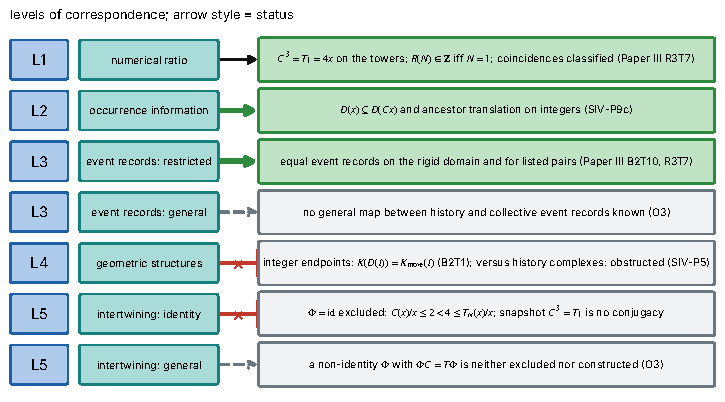
\includegraphics[width=\linewidth]{fig19_correspondence_levels.pdf}
\caption{\textbf{The five levels of cross-system correspondence.} Arrow style gives the status of what is known: established (L1), proved restricted statements (L2; L3 on the rigid domain and listed pairs), open (L3 in general; L5 for a non-identity $\Phi$), obstructed (L4 against history complexes; L5 for $\Phi=\mathrm{id}$). \emph{Schematic of status; each row cites the proposition or theorem that supports it.}}\label{fig:levels}\end{figure}
